\documentclass[12pt, a4paper]{report}

\usepackage{amsmath,amsthm,amssymb}
\usepackage{mathtext}
\usepackage[T1,T2A]{fontenc}
\usepackage[utf8]{inputenc}
\usepackage[english,russian]{babel}
\usepackage{listings}
\usepackage{graphicx}
\usepackage{indentfirst}
\usepackage{color}
\usepackage{float}
\usepackage{caption}
\captionsetup[table]{singlelinecheck=off}
\captionsetup[lstlisting]{singlelinecheck=off, labelformat=empty}
\usepackage{pgfplots}
\pgfplotsset{compat=1.9}
\usepackage[left=3cm,right=1cm, top=2cm,bottom=2cm,bindingoffset=0cm]{geometry}
\graphicspath{{./img/}}

\lstset{ 
  backgroundcolor=\color{white},   % choose the background color; you must add \usepackage{color} or \usepackage{xcolor}; should come as last argument
  breaklines=true,                 % sets automatic line breaking
  captionpos=t,                    % sets the caption-position to bottom
  commentstyle=\color{green},    % comment style
  keywordstyle=\color{blue},       % keyword style
  language=Python,                 % the language of the code
  numbers=left,                    % where to put the line-numbers; possible values are (none, left, right)
  numbersep=5pt,                   % how far the line-numbers are from the code
  numberstyle=\tiny\color{black}, % the style that is used for the line-numbers
  showspaces=false,                % show spaces everywhere adding particular underscores; it overrides 'showstringspaces'
  showstringspaces=false,          % underline spaces within strings only
  showtabs=false,                  % show tabs within strings adding particular underscores
  stepnumber=1,                    % the step between two line-numbers. If it's 1, each line will be numbered
  stringstyle=\color{yellow},     % string literal style
  tabsize=2,	                   % sets default tabsize to 2 spaces
  frame=single
}

\begin{document}

\begin{titlepage}
	\noindent \begin{minipage}{0.15\textwidth}
	
\includegraphics[width=\linewidth]{bauman_logo}
	\end{minipage}
	\footnotesize\noindent \begin{minipage}{0.8\textwidth}\centering
		\textbf{Министерство науки и высшего образования Российской Федерации}\\
		\textbf{Федеральное государственное бюджетное образовательное учреждение}\\
		\textbf{высшего образования}\\
		\textbf{~~~«Московский государственный технический университет}\\
		\textbf{имени Н.Э.~Баумана}\\
		\textbf{(национальный исследовательский университет)»}\\
		\textbf{(МГТУ им. Н.Э.~Баумана)}
	\end{minipage}
	
	\noindent\rule{17cm}{3pt}
	\newline\newline
	\large\noindent ФАКУЛЬТЕТ $\underline{\text{Информатика и системы управления}}$ \newline\newline
	\noindent КАФЕДРА $\underline{\text{Программное обеспечение ЭВМ и информационные технологии}}$\newline\newline\newline\newline\newline
	
	
	\begin{center}
		\noindent
			\LARGE\textbf{Отчёт по лабораторной работе №3}\newline
			\textbf{по дисциплине "Анализ алгоритмов"}\newline\newline
	\end{center}
	
	\large\noindent\textbf{Тема} $\underline{\text{Алгоритмы сортировки}}$\newline\newline
	\noindent\textbf{Студент} $\underline{\text{Жабин Д.В.}}$\newline\newline
	\noindent\textbf{Группа} $\underline{\text{ИУ7-54Б}}$\newline\newline
	\noindent\textbf{Преподаватель} $\underline{\text{Волкова Л.Л.}}$\newline\newline\newline
	
	\begin{center}
		\large\vfill
		Москва, 2021 г.
	\end{center}
\end{titlepage}

\setlength{\parindent}{1.25cm}

\setcounter{page}{2}\large\linespread{1.3}\tableofcontents

\newpage
\chapter*{Введение}
\addcontentsline{toc}{chapter}{Введение}

Сортировка~--- это упорядочивание элементов заданной последовательности. Работать с отсортированным списком гораздо удобнее, ведь так в разы быстрее можно найти нужный объект.

Алгоритм сортировки~--- это алгоритм для упорядочивания элементов в массиве. В случае, когда элемент в массиве имеет несколько полей, поле, служащее критерием порядка, называется ключом сортировки. На практике в качестве ключа часто выступает число, а в остальных полях хранятся какие-либо данные, никак не влияющие на работу алгоритма. Почти в каждом программном продукте используется один или даже несколько алгоритмов сортировки. 

Любой алгоритм сортировки состоит из сравнений и перестановок, количество которых определяет скорость работы алгоритма. Этот параметр является ключевым при выборе того или иного алгоритма для решения конкретной поставленной задачи.

Целью лабораторной работы является анализ алгоритмов сортировки. Для ее достижения поставлены следующие задачи:

\begin{itemize}
	\item изучить и реализовать 3 алгоритма сортировки: сортировка выбором, сортировка вставками, сортировка пузырьком;
	\item провести сравнительный анализ трудоёмкости алгоритмов на основе теоретических расчетов и выбранной модели вычислений;
	\item провести сравнительный анализ алгоритмов на основе экспериментальных данных.
\end{itemize}

\newpage
\chapter*{1 Аналитическая часть}
\addcontentsline{toc}{chapter}{1 Аналитическая часть}

Рассмотрим ключевые особенности выбранных для анализа сортировок.

\section*{1.1 Сортировка выбором}
\addcontentsline{toc}{section}{1.1. Сортировка выбором}
Алгоритм сортировки выбором работает следующим образом: находим наименьший элемент в массиве и обмениваем его с элементом находящимся на первом месте. Повторяем процесс
– находим наименьший элемент в последовательности, начиная со второго элемента, и обмениваем со вторым элементом и так далее, пока весь массив не будет отсортирован. Сортировка получила
такое название, поскольку работает, циклически выбирая наименьший из оставшихся элементов.

Главным отличием сортировки выбором от сортировки вставками является то, что в
сортировке вставками извлекается из неотсортированной части массива первый элемент (необязательно минимальный) и вставляется на своё место в отсортированной части. В сортировке выбором
при этом ищется минимальный элемент в неотсортированной части, который
вставляется в конец отсортированной части массива.


\section*{1.2 Сортировка вставками}
\addcontentsline{toc}{section}{1.2. Сортировка вставками}
Сортировка вставками~--- алгоритм сортировки, в котором элементы входной последовательности просматриваются по одному, и каждый новый поступивший элемент размещается в подходящее место среди ранее упорядоченных элементов.

Считается, что последовательность из одного элемента~--- отсортированная. Начиная со второго элемента входных данных, алгоритм помещает его на нужную позицию в уже отсортированную часть. Так до тех пор, пока весь набор входных данных не будет исчерпан [4]. В любой момент времени в отсортированной последовательности элементы удовлетворяют требованиям к выходным данным алгоритма.

\section*{1.3 Сортировка пузырьком}
\addcontentsline{toc}{section}{1.3. Сортировка пузырьком}
Алгоритм состоит из повторяющихся проходов по сортируемому массиву.
За каждый проход элементы последовательно сравниваются попарно и, если порядок в паре неверный, выполняется обмен элементов.

Проходы по массиву повторяются $N-1$ раз. При каждом проходе алгоритма по внутреннему циклу очередной наибольший элемент массива ставится на свое место в конце массива рядом с предыдущим ``наибольшим элементом'', а наименьший элемент массива перемещается на одну позицию к началу массива (``всплывает'' до нужной позиции, как пузырёк в воде~--- отсюда и название алгоритма) [4].

\section*{1.4 Вывод}
\addcontentsline{toc}{section}{1.4 Вывод}
В данном разделе были рассмотрены 3 алгоритма сортировки: сортировка выбором, сортировка вставками и сортировка пузырьком.

\newpage
\chapter*{2 Конструкторская часть}
\addcontentsline{toc}{chapter}{2 Конструкторская часть}

На основе полученных аналитических данных построим схемы алгоритмов сортировок и оценим их трудоемкости.

\section*{2.1 Схемы алгоритмов}
\addcontentsline{toc}{section}{2.1 Схемы алгоритмов}
На рисунках 2.1, 2.2 и 2.3 представлены схемы алгоритмов сортировки выбором, сортировки вставками и сортировки пузырьком соответственно.

\begin{figure}[H]
\center{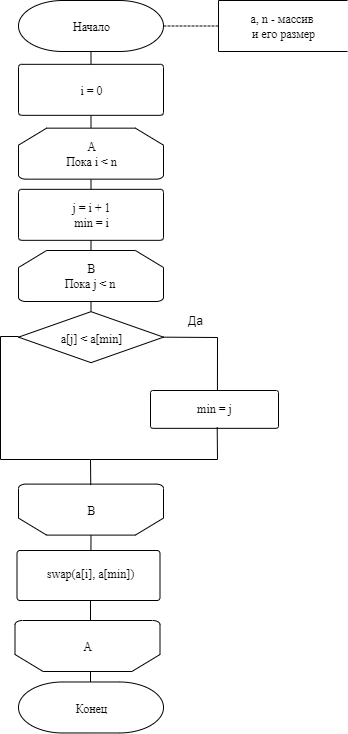
\includegraphics[scale=0.72]{select.png}}
\caption*{Рисунок 2.1~--- Сортировка выбором}
\end{figure}

\begin{figure}[H]
\center{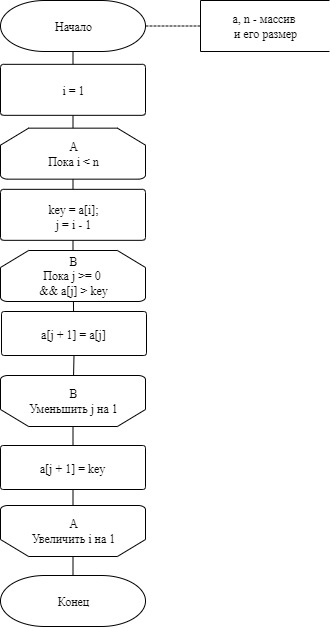
\includegraphics[scale=0.72]{insert.png}}
\caption*{Рисунок 2.2~--- Cортировка вставками}
\end{figure}

\begin{figure}[H]
\center{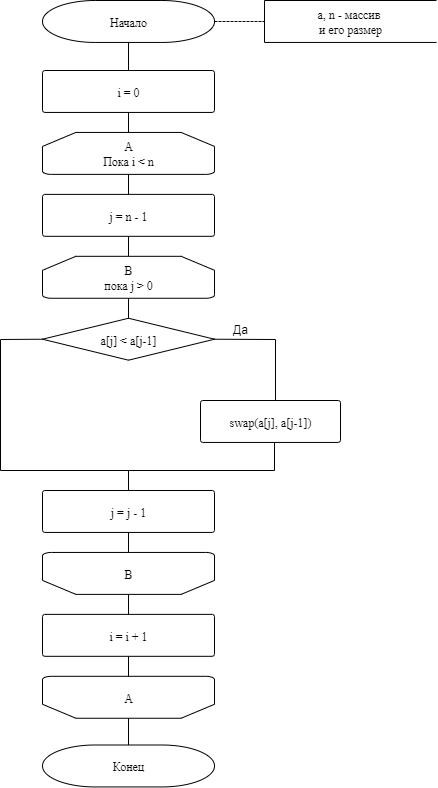
\includegraphics[scale=0.72]{bubble.png}}
\caption*{Рисунок 2.3~--- Сортировка пузырьком}
\end{figure}

\section*{2.2 Модель вычислений трудоемкости алгоритмов}
\addcontentsline{toc}{section}{2.2 Модель вычислений трудоемкости алгоритмов}

\begin{enumerate}
	\item Трудоемкость базовых операций.
	
	Трудоемкость операций из списка (2.1) равна 2. $$ *, /, \%, *=, /= \eqno (2.1)$$Операции из списка (2.2) имеют трудоемкость 1.$$=, +, -, +=, -=, ==, !=, <, >, <=, >=, ||, \&, [] \eqno (2.2)$$
	\item Трудоемкость условного оператора.
	
	Трудоемкость условного перехода равна 0, а оператора if условие then A else B рассчитывается, как (2.3) в лучшем случае и как (2.4) в худшем случае.
	$$f_{\text{if}} = f_{\text{условия}} + min(f_{\text{A}}, f_{\text{B}})\eqno (2.3)$$	$$f_{\text{if}} = f_{\text{условия}} + max(f_{\text{A}}, f_{\text{B}})\eqno (2.4)$$
	\item Трудоемкость цикла.
	
	Она рассчитывается, как (2.4).
	$$f_{\text{for}} = f_{\text{инициализации}} + f_{\text{условия}} + N(f_{\text{тела}} + f_{\text{инкремента}} + f_{\text{сравнения}})\eqno (2.4)$$
	\item Трудоемкость вызова функции равна 0.
\end{enumerate}

\section*{2.3 Трудоемкость алгоритмов}
\addcontentsline{toc}{section}{2.3 Трудоемкость алгоритмов}

Пусть размер массивов во всех вычислениях обозначается как $N$.

\subsection*{2.3.1 Алгоритм сортировки пузырьком}
\addcontentsline{toc}{subsection}{2.3.1 Алгоритм сортировки пузырьком}

Трудоёмкость алгоритма сортировки пузырьком:
\begin{itemize}
	\item трудоёмкость внешнего цикла $i \in [0..N - 1)$ : 
	$$f_{\text{i}} = 3 + (N - 1) \cdot (4 + f_{\text{j}}) \eqno (2.5)$$
	
	\item трудоёмкость внутреннего цикла $j \in[0..N - 1 - i)$ :
	$$f_{\text{j}} = 4 + (N - 1) \cdot (5 + f{\text{if}}) \eqno (2.6)$$
	
	\item трудоёмкость условия во внутреннем цикле в лучшем случае (2.7) и в худшем случае (2.8):
	$$f_{\text{ifbest}} = 4 + 0 = 4 \eqno (2.7)$$
	$$f_{\text{ifworst}} = 4 + 9 = 13 \eqno (2.8)$$
\end{itemize}

Трудоёмкость в \textbf{лучшем} случае (2.9):
$$f_{\text{best}} = 9N^2 - 10N + 4 \approx 9N^2 = O(N^2) \eqno (2.9)$$

Трудоёмкость в \textbf{худшем} случае (2.10):
$$f_{\text{worst}} = 18N^2 - 28N + 13 \approx 18N^2 = O(N^2) \eqno (2.10)$$

\subsection*{2.3.2 Алгоритм сортировки вставками}
\addcontentsline{toc}{subsection}{2.3.2 Алгоритм сортировки вставками}

Трудоёмкость алгоритма сортировки вставками:
\begin{itemize}
	\item трудоёмкость внешнего цикла $i \in [1..N)$ : 
	$$f_{\text{i}} = 2 + (N - 1) \cdot (5 + f_{\text{j}}) \eqno (2.11)$$
	
	\item трудоёмкость внутреннего цикла $j >= 0$ в лучшем случае (2.12) и в худшем случае (2.13):
	$$f_{\text{jbest}} = 5 + 0 = 5 \eqno (2.12)$$
	$$f_{\text{jworst}} = 5 + 5 \cdot (N - 1) \eqno (2.13)$$
\end{itemize}

Трудоёмкость в \textbf{лучшем} случае (2.14):
$$f_{\text{best}} = 10N - 8 \approx 10N = O(N) \eqno (2.14)$$

Трудоёмкость в \textbf{худшем} случае (2.15):
$$f_{\text{worst}} = 5N^2 - 3 \approx 5N^2 = O(N^2) \eqno (2.15)$$

\subsection*{2.3.3 Алгоритм сортировки выбором}
\addcontentsline{toc}{subsection}{2.3.3 Алгоритм сортировки выбором}

Трудоёмкость сортировки выбором в худшем и лучшем случаях совпадает и оценивается как $O(N^2)$.

\section*{2.4 Вывод}
\addcontentsline{toc}{section}{2.4 Вывод}

На основе теоретических данных, полученных из аналитического раздела, были построены схемы трёх алгоритмов сортировки. Оценены их тредёмкости в лучшем и худшем случаях.

\chapter*{3 Технологическая часть}
\addcontentsline{toc}{chapter}{3 Технологическая часть}

В данном разделе приведены средства реализации и листинги кода.

\section*{3.1 Требование к ПО}
\addcontentsline{toc}{section}{3.1 Требование к ПО}

К программе предъявляется ряд требований:

\begin{itemize}
	\item на вход ПО получает массив сравнимых элементов;
	\item на выходе~--- этот массив, отсортированный по возрастанию.
\end{itemize}

\section*{3.2 Средства реализации}
\addcontentsline{toc}{section}{3.2 Средства реализации}

Для реализации ПО был выбран язык программирования \verb|Python| [1]. Это обусловлено знанием возможностей языка, что обеспечит высокую скорость написания программы без потери ее качества. 

В качестве среды разработки выбрана \verb|Visual Studio Code| [3]. Удобства написания кода и его автодополнения стали ключевыми при выборе.

\section*{3.3 Реализация алгоритмов}
\addcontentsline{toc}{section}{3.3 Реализация алгоритмов}

В листингах 3.1 - 3.3 приведена реализация трёх алгоритмов сортировки.

\begin{lstlisting}[title=Листинг 3.1~--- Сортировка выбором]
def selection_sort(a):
    for i in range(len(a)):
        min_i = i
        for j in range(i+1, len(a)):
            if a[j] < a[min_i]:
                min_i = j
        a[min_i], a[i] = a[i], a[min_i]
    return a
\end{lstlisting}

\begin{lstlisting}[title=Листинг 3.2~--- Сортировка вставками]
def insertion_sort(a):
    for i in range(1, len(a)):
        key = a[i]
        j = i-1
        while j >= 0 and a[j] > key:
            a[j+1] = a[j]
            j -= 1
        a[j+1] = key
    return a
\end{lstlisting}

\begin{lstlisting}[title=Листинг 3.3~--- Сортировка пузырьком]
def bubble_sort(a):
    for i in range(len(a)):
        for j in range(len(a)-1, 0, -1):
            if a[j-1] > a[j]:
                a[j-1], a[j] = a[j], a[j-1]
    return a
\end{lstlisting}

\section*{3.4 Тестовые данные}
\addcontentsline{toc}{section}{3.4 Тестовые данные}

В таблице (3.1) приведены тесты для функций, реализующих алгоритмы сортировки. Все тесты пройдены успешно.

\begin{table}[h]
	\caption*{Таблица 3.1~--- Тестирование функций}
		\begin{tabular}[l]{|c|c|c|}
			\hline
			Входной массив & Результат & Ожидаемый результат \\ 
			\hline
			$[37, 44, 45, 52, 88]$ & $[37, 44, 45, 52, 88]$  & $[37, 44, 45, 52, 88]$\\\hline
			$[88, 52, 45, 44, 37]$  & $[37, 44, 45, 52, 88]$ & $[37, 44, 45, 52, 88]$\\\hline
			$[-10, -20, -30, -25, -50]$  & $[-50, -30, -25, -20, -10]$  & $[-50, -30, -25, -20, -10]$\\\hline
			$[40, -10, 20, -30, 75]$  & $[-30, -10, 20, 40, 75]$  & $[-30, -10, 20, 40, 75]$\\\hline
			$[10]$  & $[10]$  & $[10]$\\\hline
			$[-10]$  & $[-10]$  & $[-10]$\\\hline
			$[]$  & $[]$  & $[]$\\
			\hline
		\end{tabular}
\end{table}

\section*{3.5 Вывод}
\addcontentsline{toc}{section}{3.5 Вывод}

В данном разделе были разработаны исходные коды трёх алгоритмов: сортировки выбором, сортировки вставками и сортировки пузырьком.

\chapter*{4 Исследовательская часть}
\addcontentsline{toc}{chapter}{4 Исследовательская часть}

Исследуем быстродействие сортировок на практических тестах.

\section*{4.1 Технические характеристики}
\addcontentsline{toc}{section}{4.1 Технические характеристики}

Ниже приведены технические характеристики устройства, на котором было проведено тестирование ПО:

\begin{itemize}
	\item Операционная система: Windows 10 64-bit.
	\item Оперативная память: 16 GB.
	\item Процессор: Intel(R) Core(TM) i5-4690 @ 3.50GHz.
\end{itemize}

\section*{4.2 Время выполнения алгоритмов}
\addcontentsline{toc}{section}{4.2 Время выполнения алгоритмов}

Время выполнения алгоритмов замерялось с помощью специальной функции \verb|process_time()| [2] из модуля \verb|time|, которая возвращает значение в долях секунды процессорного времени текущего процесса. Контрольная точка возвращаемого значения не определена, поэтому допустима только разница между результатами последовательных вызовов.

На рисунках 4.1 - 4.3 и на графиках 4.1 - 4.3 показаны результаты замеров.

\begin{figure}[H]
\center{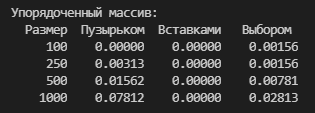
\includegraphics[scale=1]{5.png}}
\caption*{Рисунок 4.1~--- Зависимость времени выполнения алгоритмов при сортированных массивах (в секундах)}
\end{figure}

\begin{figure}[H]
\center{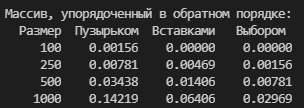
\includegraphics[scale=1]{6.png}}
\caption*{Рисунок 4.2~--- Зависимость времени выполнения алгоритмов при обратно сортированных массивах (в секундах)}
\end{figure}

\begin{figure}[H]
\center{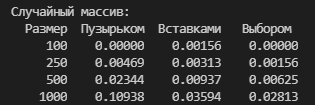
\includegraphics[scale=1]{4.png}}
\caption*{Рисунок 4.3~--- Зависимость времени выполнения алгоритмов при случайных массивах (в секундах)}
\end{figure}

\begin{figure}[H]
\center{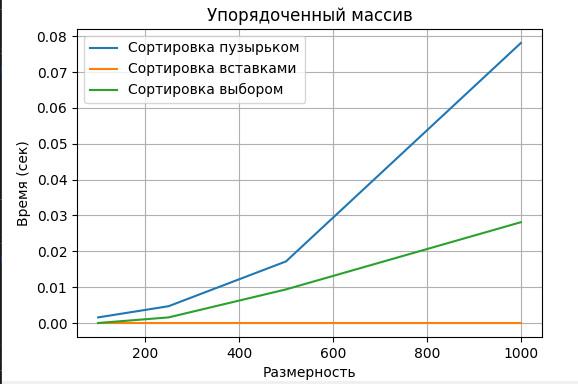
\includegraphics[scale=1]{2.png}}
\caption*{График 4.1~--- Зависимость времени выполнения от размерности при сортированных массивах}
\end{figure}

\begin{figure}[H]
\center{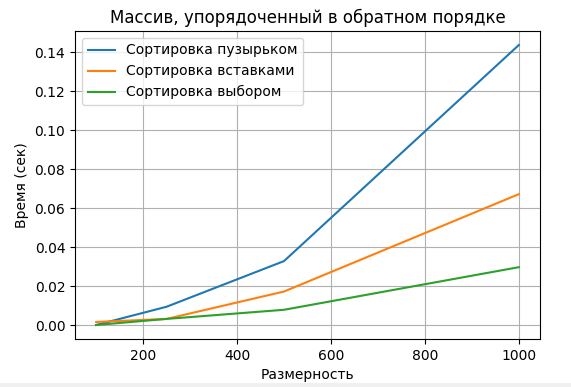
\includegraphics[scale=1]{3.png}}
\caption*{График 4.2~--- Зависимость времени выполнения от размерности при обратно сортированных массивах}
\end{figure}

\begin{figure}[H]
\center{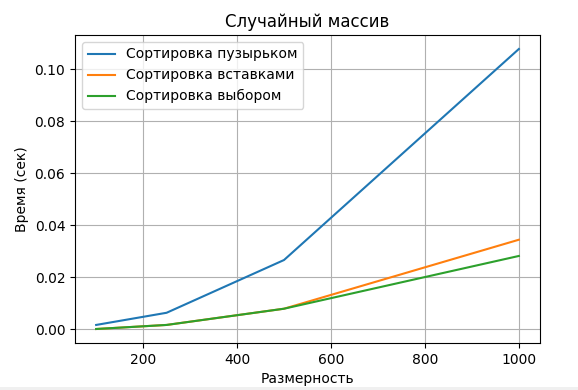
\includegraphics[scale=1]{1.png}}
\caption*{График 4.3~--- Зависимость времени выполнения от размерности при случайных массивах}
\end{figure}

\section*{4.3 Вывод}
\addcontentsline{toc}{section}{4.3 Вывод}

По результатам замеров сортировка выбором работает быстрее остальных рассмотренных сортировок, но на отсортированных массивах выигрывает сортировка вставками.
Сортировка пузырьком работает значительно медленнее на любых массивах.


\chapter*{Заключение}
\addcontentsline{toc}{chapter}{Заключение}

В ходе проделанной работы была достигнута поставленная цель и решены следующие задачи:

\begin{itemize}
	\item были изучены и реализованы 3 алгоритма сортировки: сортировка выбором, сортировка вставками, сортировка пузырьком;
	\item был проведён сравнительный анализ трудоёмкости алгоритмов на основе теоретических расчетов и выбранной модели вычислений;
	\item был проведён сравнительный анализ алгоритмов на основе экспериментальных данных.
\end{itemize}

На основании анализа трудоемкости алгоритмов в выбранной модели вычислений, было показано, что алгоритм сортировки вставками имеет трудоемкость меньше, чем другие сортировки в лучшем случае. В худшем случае все три сортировки имееют квадратическую трудоемкость. На основании замеров времени исполнения алгоритмов, был сделан вывод, что сортировка выбором имеет наименьшее время работы на случайных и обратно сортированных массивах. Также была доказана выведенная трудоемкость алгоритма сортировки пузырьком~--- на любых данных имеет сложность $O(N^2)$.

\chapter*{Литература}
\addcontentsline{toc}{chapter}{Литература}

[1] Python [Электронный ресурс]. Режим доступа: https://python.org. Дата обращения: 17.10.2021.\\

[2] Модуль time [Электронный ресурс]. Режим доступа: \newline https://docs.python.org/3/library/time.html. Дата обращения: 17.10.2021.\\

[3] Visual Studio Code - Code Editing [Электронный ресурс]. Режим доступа: \newline https://code.visualstudio.com. Дата обращения: 17.10.2021.\\

[4] Сортировки [Электронный ресурс]. Режим доступа: \newline https://function-x.ru/cpp-algoritmy-sortirovki.html. Дата обращения: 17.10.2021.

\end{document}